\documentclass[a4paper, 10pt]{article}
\usepackage[english]{babel}
\usepackage[utf8]{inputenc}
\usepackage{enumitem}
\usepackage{titlesec}
\usepackage{framed}
\usepackage{listings}
\usepackage{graphicx}
\usepackage{titling}
\usepackage{blindtext}
\usepackage{amsmath}  % for \hookrightarrow
\usepackage{xcolor}   % for \textcolor
\graphicspath{ {./ER/} }
\usepackage[hmargin=2cm,vmargin=3.5cm,bmargin=2cm]{geometry}

\setlist[itemize]{noitemsep, topsep=0pt}
\setlength\parindent{0pt}

\setcounter{secnumdepth}{0} %% no numbering

\begin{document}
\title{Advanced DataBases C4 Group\\\
  \huge Bank Management System}
\author{
  Samuel Lúcio Vicente, 251720
  \and
  Daniel Silva, 251702
  \and
  Jorge Marrero Camiruaga, 251438
}

\date{Politechnika Wrocławska\\today}

\maketitle

\lstset{
  basicstyle=\small\ttfamily,
  frame=lrtb,
  numbers=left,
  columns=fullflexible,
  breaklines=true,
  postbreak=\mbox{\textcolor{red}{$\hookrightarrow$}\space}
}

\section{Short Description}
This database models a bank with Accounts that can either be a SavingsAccount or a CurrentAccount. There are some operations that are permitted, Withdraw from the CurrentAccount, Transfer between accounts, Loan, Pay the loan, Deposit on Account. There are employees that work in a branch that have roles, this database tracks the history of theall the employees on every branch, and the previous roles that some particular employee has had and which branch he has working at.

\section{ERD}
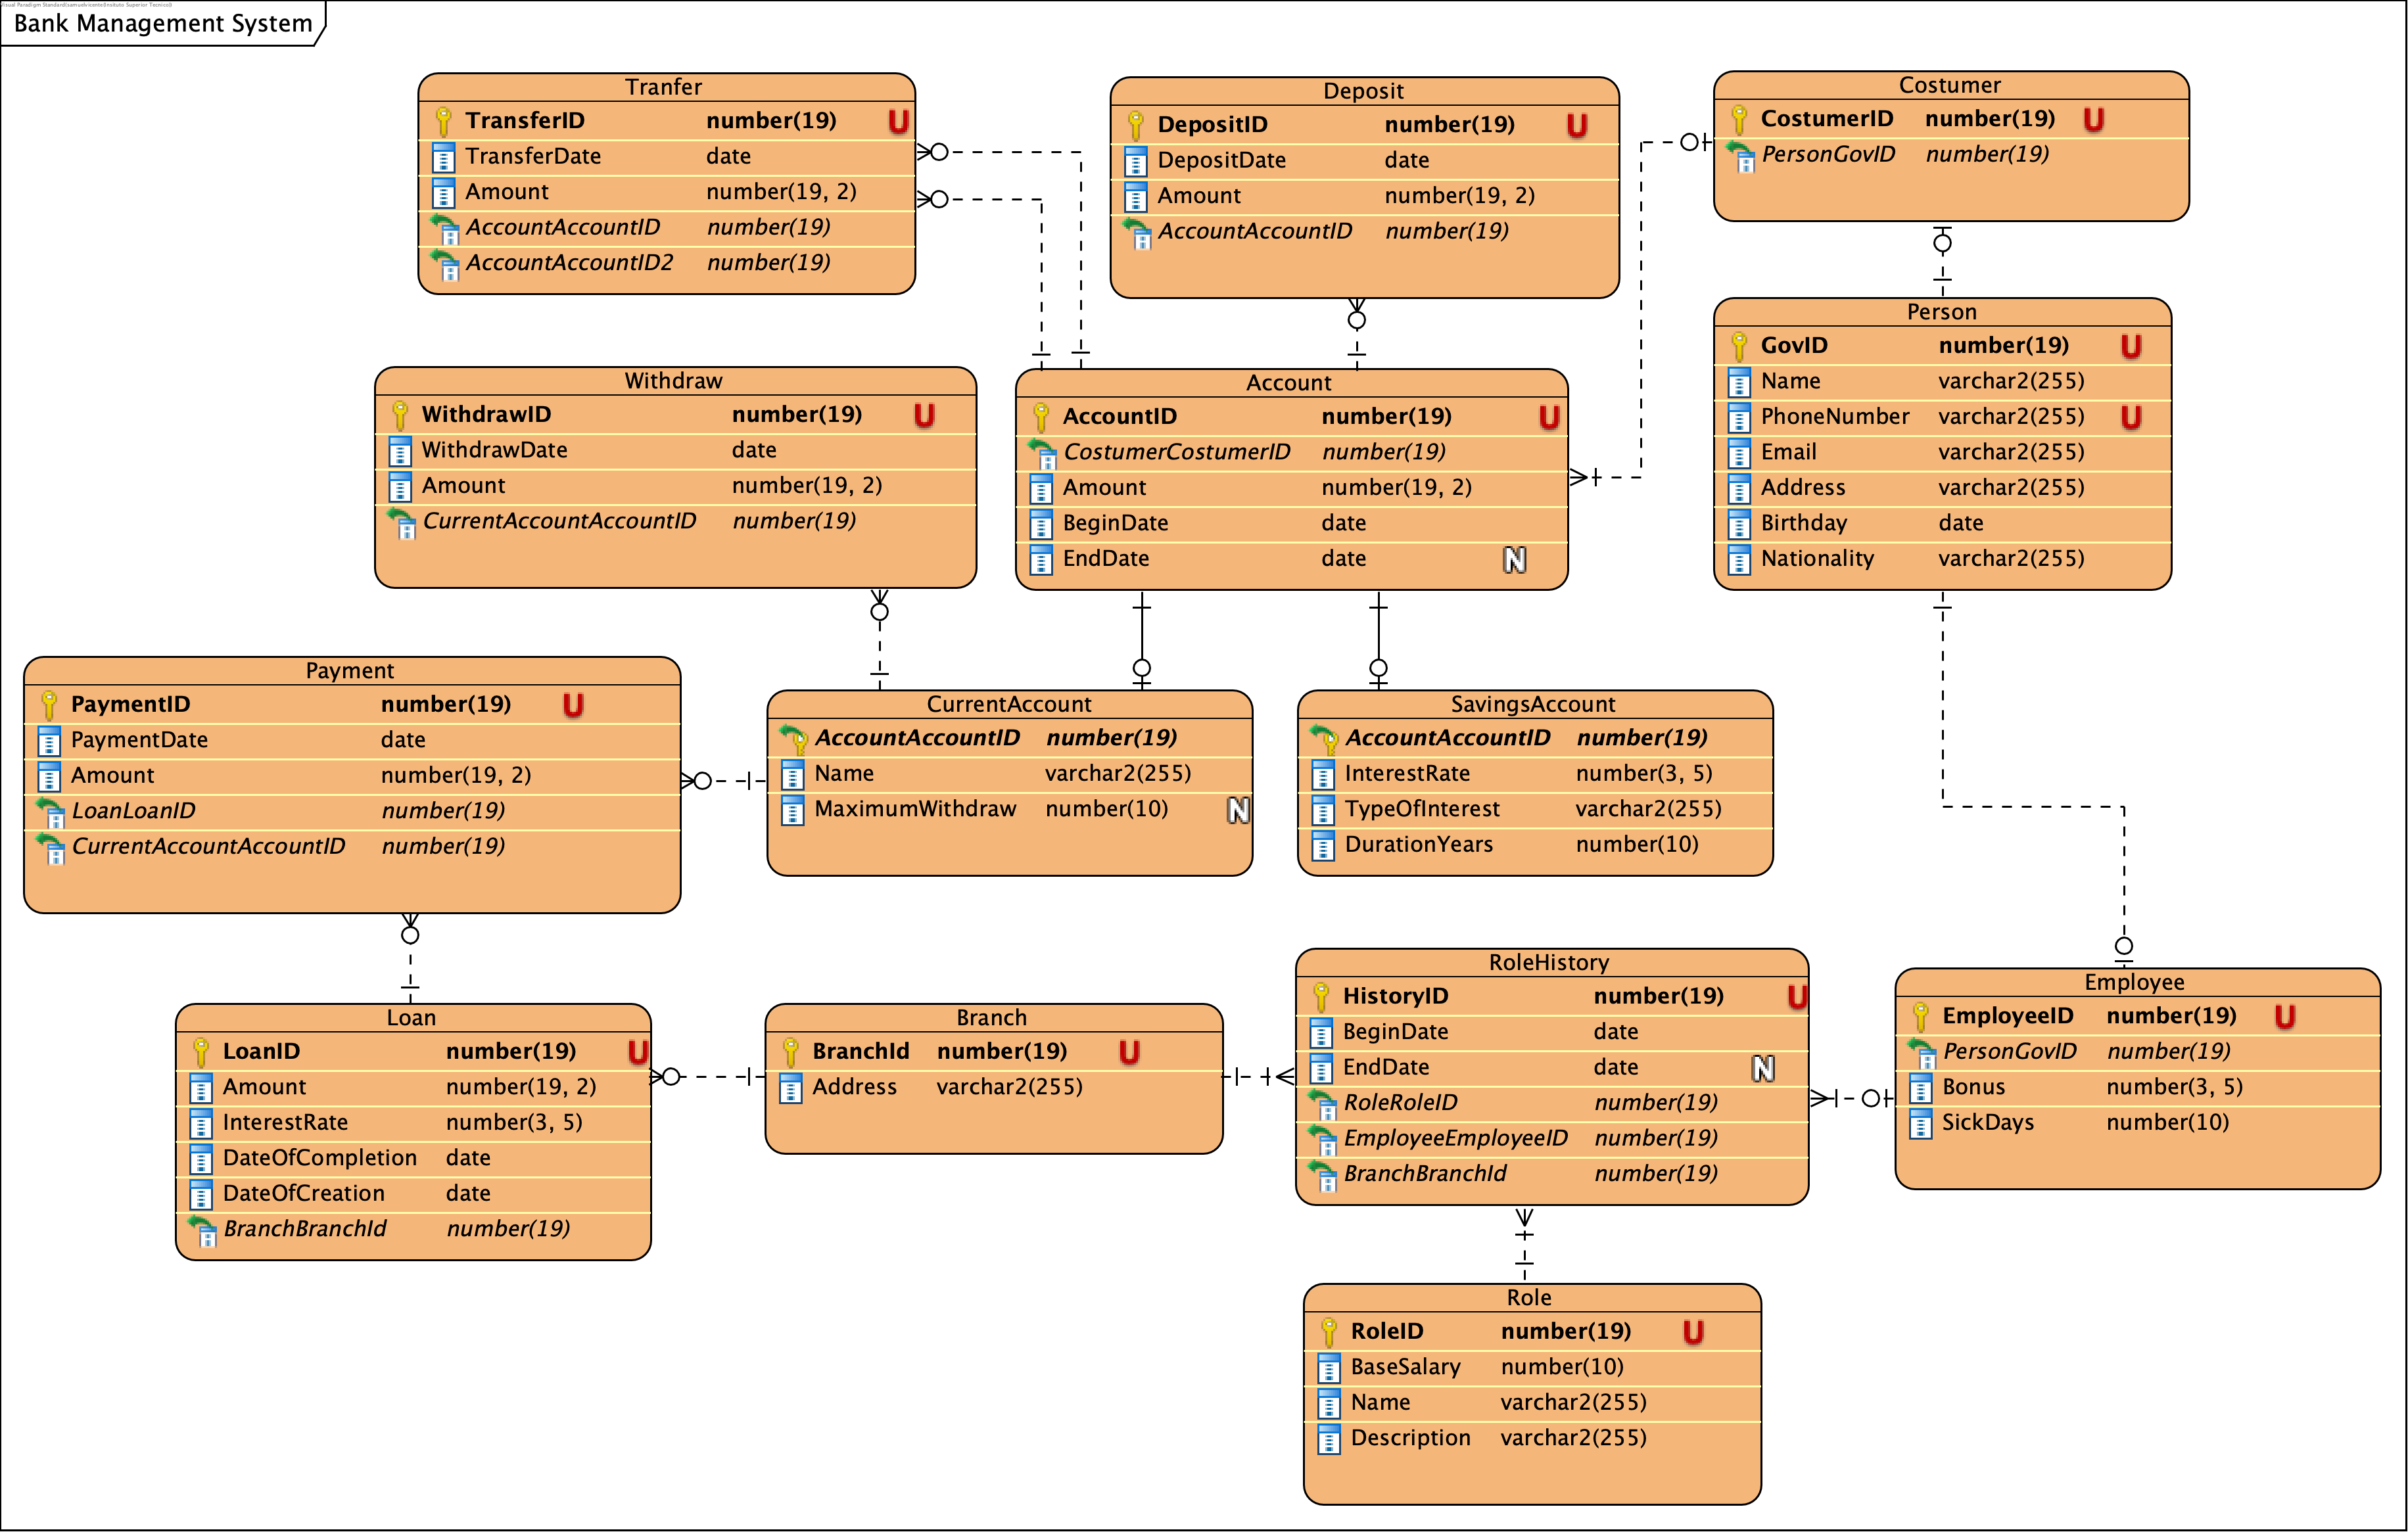
\includegraphics[width=\textwidth,height=\textheight,keepaspectratio]{bms}
\section{Schema}
\begin{lstlisting}[language=SQL]
CREATE TABLE Person (
  GovID       number(19) GENERATED AS IDENTITY, 
  Name        varchar2(255) NOT NULL, 
  PhoneNumber varchar2(255) NOT NULL UNIQUE, 
  Email       varchar2(255) NOT NULL, 
  Address     varchar2(255) NOT NULL, 
  Birthday    date NOT NULL, 
  Nationality varchar2(255) NOT NULL, 
  PRIMARY KEY (GovID));

CREATE TABLE Costumer (
  CostumerID  number(19) GENERATED AS IDENTITY, 
  PersonGovID number(19) NOT NULL, 
  PRIMARY KEY (CostumerID));

CREATE TABLE Employee (
  EmployeeID  number(19) GENERATED AS IDENTITY, 
  PersonGovID number(19) NOT NULL, 
  Bonus       number(3, 5) NOT NULL CHECK(Bonus>=0), 
  SickDays    number(10) NOT NULL CHECK(SickDays<10), 
  PRIMARY KEY (EmployeeID));

CREATE TABLE Account (
  AccountID          number(19) GENERATED AS IDENTITY, 
  CostumerCostumerID number(19) NOT NULL, 
  Amount             number(19, 2) NOT NULL CHECK(Amount>=0), 
  BeginDate          date NOT NULL, 
  EndDate            date, 
  PRIMARY KEY (AccountID));

CREATE TABLE Branch (
  BranchId number(19) GENERATED AS IDENTITY, 
  Address  varchar2(255) NOT NULL, 
  PRIMARY KEY (BranchId));

CREATE TABLE RoleHistory (
  HistoryID          number(19) GENERATED AS IDENTITY, 
  BeginDate          date NOT NULL, 
  EndDate            date, 
  RoleRoleID         number(19) NOT NULL, 
  EmployeeEmployeeID number(19) NOT NULL, 
  BranchBranchId     number(19) NOT NULL, 
  PRIMARY KEY (HistoryID));

CREATE TABLE Role (
  RoleID      number(19) GENERATED AS IDENTITY, 
  BaseSalary  number(10) NOT NULL CHECK(BaseSalary>0), 
  Name        varchar2(255) NOT NULL, 
  Description varchar2(255) NOT NULL, 
  PRIMARY KEY (RoleID));

CREATE TABLE Loan (
  LoanID           number(19) GENERATED AS IDENTITY, 
  Amount           number(19, 2) NOT NULL CHECK(Amount>0), 
  InterestRate     number(3, 5) NOT NULL, 
  DateOfCompletion date NOT NULL, 
  DateOfCreation   date NOT NULL, 
  BranchBranchId   number(19) NOT NULL, 
  PRIMARY KEY (LoanID));

CREATE TABLE Payment (
  PaymentID               number(19) GENERATED AS IDENTITY, 
  PaymentDate             date NOT NULL, 
  Amount                  number(19, 2) NOT NULL CHECK(Amount>0), 
  LoanLoanID              number(19) NOT NULL, 
  CurrentAccountAccountID number(19) NOT NULL, 
  PRIMARY KEY (PaymentID));

CREATE TABLE SavingsAccount (
  AccountAccountID number(19) NOT NULL, 
  InterestRate     number(3, 5) NOT NULL CHECK(InterestRate>0), 
  TypeOfInterest   varchar2(255) NOT NULL, 
  DurationYears    number(10) NOT NULL CHECK(DurationYears>0), 
  PRIMARY KEY (AccountAccountID));

CREATE TABLE Deposit (
  DepositID        number(19) GENERATED AS IDENTITY, 
  DepositDate      date NOT NULL, 
  Amount           number(19, 2) NOT NULL CHECK(Amount>0), 
  AccountAccountID number(19) NOT NULL, 
  PRIMARY KEY (DepositID));

CREATE TABLE Transfer (
  TransferID        number(19) GENERATED AS IDENTITY, 
  TransferDate      date NOT NULL, 
  Amount            number(19, 2) NOT NULL CHECK(Amount>0), 
  AccountAccountID  number(19) NOT NULL, 
  AccountAccountID2 number(19) NOT NULL, 
  PRIMARY KEY (TransferID));

CREATE TABLE Withdraw (
  WithdrawID              number(19) GENERATED AS IDENTITY, 
  WithdrawDate            date NOT NULL, 
  Amount                  number(19, 2) NOT NULL CHECK(Amount>0), 
  CurrentAccountAccountID number(19) NOT NULL, 
  PRIMARY KEY (WithdrawID));

CREATE TABLE CurrentAccount (
  AccountAccountID number(19) NOT NULL, 
  Name             varchar2(255) NOT NULL, 
  MaximumWithdraw  number(10), 
  PRIMARY KEY (AccountAccountID));

ALTER TABLE Costumer ADD CONSTRAINT FKCostumer923053 FOREIGN KEY (PersonGovID) REFERENCES Person (GovID);

ALTER TABLE Employee ADD CONSTRAINT FKEmployee249023 FOREIGN KEY (PersonGovID) REFERENCES Person (GovID);

ALTER TABLE Account ADD CONSTRAINT FKAccount895601 FOREIGN KEY (CostumerCostumerID) REFERENCES Costumer (CostumerID);

ALTER TABLE RoleHistory ADD CONSTRAINT FKRoleHistor647811 FOREIGN KEY (RoleRoleID) REFERENCES Role (RoleID);

ALTER TABLE RoleHistory ADD CONSTRAINT FKRoleHistor516821 FOREIGN KEY (EmployeeEmployeeID) REFERENCES Employee (EmployeeID);

ALTER TABLE RoleHistory ADD CONSTRAINT FKRoleHistor171832 FOREIGN KEY (BranchBranchId) REFERENCES Branch (BranchId);

ALTER TABLE Loan ADD CONSTRAINT FKLoan357293 FOREIGN KEY (BranchBranchId) REFERENCES Branch (BranchId);

ALTER TABLE SavingsAccount ADD CONSTRAINT FKSavingsAcc25288 FOREIGN KEY (AccountAccountID) REFERENCES Account (AccountID);

ALTER TABLE Payment ADD CONSTRAINT FKPayment955503 FOREIGN KEY (LoanLoanID) REFERENCES Loan (LoanID);

ALTER TABLE Deposit ADD CONSTRAINT FKDeposit626030 FOREIGN KEY (AccountAccountID) REFERENCES Account (AccountID);

ALTER TABLE Transfer ADD CONSTRAINT FKTranfer816388 FOREIGN KEY (AccountAccountID) REFERENCES Account (AccountID);

ALTER TABLE Transfer ADD CONSTRAINT FKTranfer299653 FOREIGN KEY (AccountAccountID2) REFERENCES Account (AccountID);

ALTER TABLE Payment ADD CONSTRAINT FKPayment25568 FOREIGN KEY (CurrentAccountAccountID) REFERENCES CurrentAccount (AccountAccountID);

ALTER TABLE Withdraw ADD CONSTRAINT FKWithdraw546165 FOREIGN KEY (CurrentAccountAccountID) REFERENCES CurrentAccount (AccountAccountID);

ALTER TABLE CurrentAccount ADD CONSTRAINT FKCurrentAcc16041 FOREIGN KEY (AccountAccountID) REFERENCES Account (AccountID);
\end{lstlisting}

\section{Transactions}

\subsection{1:Changing Query}
\subsubsection{Description}
There is 5 CurrentAccount in the system. This transaction doubles the amount of the account that has the biggest value in the database.

\subsubsection{SQL}
\begin{lstlisting}[language=SQL]
BEGIN TRANSACTION
UPDATE Account 
SET amount = amount*2 
WHERE AccountID = (
    SELECT AccountID 
    FROM Costumer c 
    INNER JOIN Person p 
        ON p.GovID = c.PersonGovID 
    INNER JOIN Account 
        ON CostumerID = CostumerCostumerID 
    INNER JOIN CurrentAccount 
        ON AccountAccountID = AccountID 
    WHERE amount >= ALL(
        SELECT MAX(amount) 
        FROM Account 
    )
);
COMMIT
\end{lstlisting}

\subsection{2:Changing Query}
\subsubsection{Description}
This transaction preforms a withdraw of 100 units on the CurrentAccount with the AccountAccountID 1. To do this we must first check if the amount we want to withdraw is smaller than the CurrentAccount MaximumWithdraw, after that we update the amount and add an entry to the Withdraw ledger.

\subsubsection{SQL}
\begin{lstlisting}[language=SQL]
BEGIN TRANSACTION
UPDATE Account
SET amount =
    CASE 
        WHEN 100<(
            SELECT MaximumWithdraw 
            FROM CurrentAccount 
            WHERE AccountAccountID=1) 
          THEN amount - 100
        ELSE amount
    END
WHERE AccountID=(
    SELECT AccountID 
    FROM CurrentAccount INNER JOIN Account 
        ON AccountID=AccountAccountID 
    WHERE AccountAccountID=1);

UPDATE Account
SET EndDate =
    CASE 
        WHEN amount=0 THEN CURRENT_DATE
        ELSE null
    END
WHERE AccountID = (
    SELECT AccountID 
    FROM CurrentAccount INNER JOIN Account 
        ON AccountID=AccountAccountID 
    WHERE AccountAccountID=1);

INSERT INTO Withdraw(WithdrawDate, Amount, CurrentAccountAccountID) VALUES(CURRENT_DATE, 100, 1);
COMMIT
\end{lstlisting}

\subsection{3:Changing Query}
\subsubsection{Description}
This transaction preforms a transaction between the SavingsAccount 6 and the CurrentAccount 1, it checks if the period of the SavingsAccount has passed and if so transfers the amount plus interest, if not only the amount. To do this we first add the amount to the CurrentAccount then we add a entry to the Transaction ledger and then we update the amount on the SavingsAccount

\subsubsection{SQL}
\begin{lstlisting}[language=SQL]
BEGIN TRANSACTION
UPDATE Account 
SET amount =     
  CASE          
      WHEN (
      SELECT EXTRACT(YEAR FROM CURRENT_DATE) - EXTRACT(YEAR FROM (
          SELECT BeginDate 
          FROM Account INNER JOIN SavingsAccount 
            ON AccountID=AccountAccountID 
          WHERE AccountAccountID=7))
        AS year FROM dual) > (
          SELECT DurationYears 
          FROM SavingsAccount 
          WHERE AccountAccountID=7)
      THEN amount + ( 
          SELECT (amount+1)*12*DurationYears*InterestRate 
          FROM  SavingsAccount INNER JOIN Account 
          ON AccountID=AccountAccountID 
          WHERE AccountAccountID=7)   
      ELSE amount + ( 
      SELECT amount 
      FROM  SavingsAccount INNER JOIN Account 
      ON AccountID=AccountAccountID 
      WHERE AccountAccountID=7) 
  END 
WHERE AccountID = (
    SELECT AccountID 
    FROM CurrentAccount INNER JOIN Account 
        ON AccountID=AccountAccountID 
    WHERE AccountAccountID=1);

INSERT INTO Transfer(TransferDate, Amount, AccountAccountID, AccountAccountID2) VALUES (CURRENT_DATE, (
Select
  CASE
      WHEN (
          SELECT EXTRACT(YEAR FROM CURRENT_DATE) - EXTRACT(YEAR FROM (
              SELECT BeginDate 
              FROM Account INNER JOIN SavingsAccount 
                ON AccountID=AccountAccountID WHERE AccountAccountID=7)) 
          AS year FROM dual) > (
              SELECT DurationYears 
              FROM SavingsAccount 
              WHERE AccountAccountID=7)
      THEN  amount*12*DurationYears*InterestRate
      ELSE  amount
  END
FROM SavingsAccount INNER JOIN Account
        ON AccountID=AccountAccountID
    WHERE AccountAccountID=7), '7', '1');

UPDATE Account
SET amount = 0
WHERE AccountID = (
    SELECT AccountID 
    FROM SavingsAccount INNER JOIN Account 
        ON AccountID=AccountAccountID 
    WHERE AccountAccountID=7);
COMMIT
\end{lstlisting}

\subsection{4:Changing Query}
\subsubsection{Description}
This transaction upgrades the role of the employee that has been working as a 4 Role for the longest time and upgrades him to a 5

\subsubsection{SQL}
\begin{lstlisting}[language=SQL]
BEGIN TRANSACTION
UPDATE RoleHistory
	SET EndDate = CURRENT_DATE
		WHERE EmployeeEmployeeID = (
				SELECT EmployeeEmployeeID 
				FROM RoleHistory
				WHERE BeginDate = (
          SELECT MIN(BeginDate)
				  FROM roleHistory
				  WHERE RoleRoleID = '4' AND EndDate = NULL)
        AND RoleRoleID = '4' AND EndDate = NULL

INSERT INTO RoleHistory VALUES('10004',CURRENT_DATE,NULL,'5','84972','16516');
COMMIT
\end{lstlisting}

\subsection{5:Changing Query}
\subsubsection{Description}
This transaction doubles the amount of every Account belonging to a Portuguese or a Spanish person

\subsubsection{SQL}
\begin{lstlisting}[language=SQL]
BEGIN TRANSACTION 
UPDATE RoleHistory 
  SET EndDate = CURRENT_DATE 
  WHERE EmployeeEmployeeID = (
    SELECT EmployeeEmployeeID 
    FROM RoleHistory 
    WHERE BeginDate = ( 
      SELECT MIN(BeginDate) 
      FROM roleHistory 
        WHERE RoleRoleID = '4' 
          AND EndDate = NULL) 
      AND RoleRoleID = '4' 
      AND EndDate = NULL 

INSERT INTO RoleHistory VALUES('10004',CURRENT_DATE,NULL,'5','84972','16516');
COMMIT
\end{lstlisting}

\subsection{6:Selecting Query}
\subsubsection{Description}
This query selects the AccountAccountID that made the transactions with the most total value
\subsubsection{SQL}
\begin{lstlisting}[language=SQL]
Select AccountAccountID, MAX(total) as TotalTransfer
FROM (
	Select TransferID,
	SUM (Amount) as total,
	From Transfer
	Group by AccountAccountID
)
\end{lstlisting}

\subsection{7:Selecting Query}
\subsubsection{Description}
This query finds the biggest amount that a costumer has on the bank
\subsubsection{SQL}
\begin{lstlisting}[language=SQL]
SELECT MAX(SUM(amount))
FROM Costumer INNER JOIN Account 
  ON CostumerCostumerID = CostumerID
GROUP BY CostumerID
\end{lstlisting}

\end{document}
